\chapter{背景知识}

\section{偏序集}

集合 $S$ 若配备二元关系 $\preccurlyeq$ 而成为偏序集，则对任意 $a,b,c \in  S$ ，均有

(i) $a \preccurlyeq  a$ ,

(ii) $a \preccurlyeq  b$ 且 $b \preccurlyeq  a$ 蕴含 $a = b$ ，

(iii) $a \preccurlyeq  b$ 且 $b \preccurlyeq  c$ 蕴含 $a \preccurlyeq  c$ .

偏序集 $S$ 的子集 ${S}^{\prime } \subseteq  S$ 称为全序的，若对任意 $a,b \in  {S}^{\prime }$ ，总有 $a \preccurlyeq  b$ 或 $b \preccurlyeq  a$ 成立.若 ${S}^{\prime }$ 不被任何其他全序集真包含，则称该子集 ${S}^{\prime }$ 为极大(关于全序性而言).

利用Zorn引理或选择公理，可证得

\begin{theorem}[Hausdorff极大性原理]\label{thm:app-A-1}
若 $S$ 为任意偏序集，则其任一全序子集 ${S}^{\prime } \subseteq  S$ 均包含于某个极大全序子集中.
\end{theorem}

\section{度量空间与拓扑空间}

集合 $X$ 上的距离是指满足以下三条性质的映射 $d : X \times  X \mapsto  {\mathbb{R}}_{ + }$ :

(1) 正定性: $d\left( {x,y}\right)  \geq  0,d\left( {x,y}\right)  = 0$ 当且仅当 $x = y$ ，

(2) 对称性: $d\left( {x,y}\right)  = d\left( {y,x}\right)$ ，

(3) 三角不等式: $d\left( {x,z}\right)  \leq  d\left( {x,y}\right)  + d\left( {y,z}\right)$ .

配备距离函数 $d\left( {\cdot , \cdot  }\right)$ 的集合 $X$ 称为度量空间.

以点 $x$ 为中心、半径为 $r > 0$ 的开球是如下集合

\[
B\left( {x,r}\right)  \doteq  \{ y \in  X;d\left( {y,x}\right)  < r\} .
\]

反过来，度量 $d\left( {\cdot , \cdot  }\right)$ 在 $X$ 上确定一个拓扑.

子集 $A \subseteq  X$ 是开集，若对每个 $x \in  A$ ，均存在半径 $r > 0$ ，使得 $B\left( {x,r}\right)  \subseteq  A$ .

子集 $C \subseteq  X$ 是闭集，若其补集 $X \setminus  C = \{ x \in  X;x \notin  C\}$ 是开集.

若 $B\left( {x,r}\right)  \subseteq  A$ 对某个 $r > 0$ 成立，则称 $A$ 是点 $x$ 的邻域，或等价地称 $x$ 是 $A$ 的内点.

— 任意一族开集的并集是开集；有限个开集的交集是开集.

— 任意一族闭集的交集是闭集；有限个闭集的并集是闭集.

全空间 $X$ 和空集 $\varnothing$ 恒既开又闭.若不存在其他同时既开又闭的子集 $S \subset  X$ ，则称空间 $X$ 是连通的.

序列 ${\left( {x}_{n}\right) }_{n \geq  1}$ 收敛于点 $x \in  X$ ，若
\[
\mathop{\lim }\limits_{{n \rightarrow  \infty }}d\left( {{x}_{n},x}\right)  = 0.
\]

此时记作 $\mathop{\lim }\limits_{{n \rightarrow  \infty }}{x}_{n} = x$ ，或简记为 ${x}_{n} \rightarrow  x$ .

集合 $A$ 的闭包记为 $\bar{A}$ ，是包含 $A$ 的最小闭集；它由所有包含 $A$ 的闭集之交给出.点 $x$ 属于集合 $A$ 的闭包，当且仅当存在一列点 ${x}_{n} \in  A$ 收敛于 $x$ .

子集 $S \subseteq  X$ 在 $X$ 中稠密，若 $\bar{S} = X$ .这等价于: $S$ 与 $X$ 的每个非空开子集均相交.若空间 $X$ 含有可数稠密子集，则称其为可分的.

序列 ${\left( {x}_{n}\right) }_{n \geq  1}$ 是Cauchy序列，如果对任意 $\varepsilon  > 0$ ，存在足够大的整数 $N$ ，使得
\[
d\left( {{x}_{m},{x}_{n}}\right)  \leq  \varepsilon \;\text{当}\; m,n \geq  N.
\]

度量空间 $X$ 是完备的，如果每个Cauchy序列都收敛于某个极限点 $x \in  X$ .

若 $X,Y$ 是两个度量空间，则映射 $f : X \mapsto  Y$ 连续，当且仅当对每个开集 $A \subseteq  Y$，其原像 ${f}^{-1}\left( A\right)  \doteq  \{ x \in  X;f\left( x\right)  \in  A\}$ 是 $X$ 中的开子集.

映射 $f : X \mapsto  Y$ 连续当且仅当，对每个 ${x}_{0} \in  X$ 和 $\varepsilon  > 0$ ，存在 $\delta  > 0$ ，使得
\[
d\left( {x,{x}_{0}}\right)  < \delta \;\implies \;d\left( {f\left( x\right) ,f\left( {x}_{0}\right) }\right)  < \varepsilon .
\]

我们称函数 $f : X \mapsto  Y$ 是Lipschitz连续的，如果存在常数 $C \geq  0$ ，使得
\[
d\left( {f\left( x\right) ,f\left( {x}^{\prime }\right) }\right)  \leq  C \cdot  d\left( {x,{x}^{\prime }}\right) \;\forall\,x,{x}^{\prime } \in  X.
\]

更一般地，我们称 $f : X \mapsto  Y$ 是指数为 $0 < \alpha  \leq  1$ 的Hölder连续函数，如果存在常数 $C$ ，使得
\[
d\left( {f\left( x\right) ,f\left( {x}^{\prime }\right) }\right)  \leq  C \cdot  {\left(  d\left( x,{x}^{\prime }\right) \right)  }^{\alpha }\;\forall\,x,{x}^{\prime } \in  X.
\]

一族满足 $K \subseteq  \mathop{\bigcup }\limits_{{i \in  \mathcal{I}}}{A}_{i}$ 的开集 $\left\{  {{A}_{i};i \in  \mathcal{I}}\right\}$ 称为集合 $K$ 的一个开覆盖.此处指标集 $\mathcal{I}$ 可以是无限的.集合 $K \subseteq  X$ 是紧的，如果对 $K$ 的任意开覆盖，均可提取出一个有限子覆盖.

集合 $S$ 是相对紧的，如果其闭包 $\bar{S}$ 是紧的.

集合 $S$ 是预紧的，如果对任意 $\varepsilon  > 0$ ，它可被有限个半径为 $\varepsilon$ 的球所覆盖.

\begin{theorem}[${\mathbb{R}}^{n}$ 中的紧子集]\label{thm:app-A-2}
子集 $S \subset  {\mathbb{R}}^{n}$ 是紧的当且仅当它既闭又有界.
\end{theorem}

\begin{theorem}[紧性的等价刻画]\label{thm:app-A-3}
设 $S$ 是一个度量空间.以下命题等价:

(i) $S$ 是紧的.

(ii) $S$ 是预紧的且完备的.

(iii) 对 $S$ 中任意点列 ${\left( {x}_{k}\right) }_{k \geq  1}$ ，均可提取出一个收敛于某极限点 $x \in  S$ 的子列.
\end{theorem}

\subsection{压缩映射的不动点}
设 $\phi  : X \mapsto  X$是从完备度量空间 $X$ 到其自身的映射.满足$\phi \left( {x}^{ * }\right)  = {x}^{ * }$ 的点 ${x}^{ * }$ 称为 $\phi$ 的不动点.对严格压缩映射，该不动点唯一，且可通过简单的迭代程序得到.

\begin{theorem}[压缩映射定理]\label{thm:app-A-4}
设 $X$ 是一个完备度量空间， $\phi  : X \mapsto  X$ 是一个连续映射，且对某个 $\kappa  < 1$ ，有
\begin{equation}\tag{A.1}\label{eq:app-A-1}
d\left( {\phi \left( x\right) ,\phi \left( y\right) }\right)  \leq  {\kappa d}\left( {x,y}\right) \;\forall\,x,y \in  X.
\end{equation}

此时存在唯一一点 ${x}^{ * } \in  X$ ，使得
\begin{equation}\tag{A.2}\label{eq:app-A-2}
{x}^{ * } = \phi \left( {x}^{ * }\right) .
\end{equation}

此外，对任意 $y \in  X$ ，均有
\begin{equation}\tag{A.3}\label{eq:app-A-3}
d\left( {y,{x}^{ * }}\right)  \leq  \frac{1}{1 - \kappa }d\left( {y,\phi \left( y\right) }\right) .
\end{equation}
\end{theorem}

\begin{proof}
任取一点 $y \in  X$ ，并考虑序列
\[
{y}_{0} = y,\;{y}_{1} = \phi \left( {y}_{0}\right) ,\;\ldots ,\;{y}_{n + 1} = \phi \left( {y}_{n}\right) ,\;\ldots
\]

由归纳法可得
{\setjot[-2]\begin{gather*}
    d\left( {{y}_{2},{y}_{1}}\right)  \leq  {\kappa d}\left( {{y}_{1},{y}_{0}}\right)\\
    d\left( {{y}_{3},{y}_{2}}\right)  \leq  {\kappa d}\left( {{y}_{2},{y}_{1}}\right)  \leq  {\kappa }^{2}d\left( {{y}_{1},{y}_{0}}\right)\\
    \cdots \\
d\left( {{y}_{n + 1},{y}_{n}}\right)  \leq  {\kappa d}\left( {{y}_{n},{y}_{n - 1}}\right)  \leq  {\kappa }^{n}d\left( {{y}_{1},{y}_{0}}\right)  = {\kappa }^{n}d\left( {\phi \left( y\right) ,y}\right) .
\end{gather*}}

在$m < n$ 处有
\begin{equation}\tag{A.4}\label{eq:app-A-4}
d\left( {{y}_{n},{y}_{m}}\right)  \leq  \sum_{{j = m}}^{{n - 1}}d\left( {{y}_{j + 1},{y}_{j}}\right)  \leq  \sum_{{j = m}}^{{n - 1}}{\kappa }^{j}d\left( {y,\phi \left( y\right) }\right)  \leq  \frac{{\kappa }^{m}}{1 - \kappa }d\left( {y,\phi \left( y\right) }\right) .
\end{equation}

由于 $\kappa  < 1$ ，\eqref{eq:app-A-4}式右端当 $m \rightarrow  \infty$ 时趋于零，故序列 ${\left( {y}_{n}\right) }_{n \geq  1}$ 为Cauchy列.又因 $X$ 完备，该序列收敛于某极限点 ${x}^{ * }$ .由 $\phi$ 的连续性可得
\[
{x}^{ * } = \mathop{\lim }\limits_{{n \rightarrow  \infty }}{y}_{n} = \mathop{\lim }\limits_{{n \rightarrow  \infty }}\phi \left( {y}_{n - 1}\right)  = \phi \left( {\mathop{\lim }\limits_{{n \rightarrow  \infty }}{y}_{n - 1}}\right)  = \phi \left( {x}^{ * }\right)
\]

因而\eqref{eq:app-A-2}成立.不动点 ${x}^{ * }$ 的唯一性证明如下:若
\[
{x}_{1} = \phi \left( {x}_{1}\right) ,\;{x}_{2} = \phi \left( {x}_{2}\right) ,
\]

则由\eqref{eq:app-A-1}可得
\[
d\left( {{x}_{1},{x}_{2}}\right)  = d\left( {\phi \left( {x}_{1}\right) ,\phi \left( {x}_{2}\right) }\right)  \leq  {\kappa d}\left( {{x}_{1},{x}_{2}}\right) .
\]

$\kappa  < 1$ 的假设从而推出 $d\left( {{x}_{1},{x}_{2}}\right)  = 0$ ，进而推出 ${x}_{1} = {x}_{2}$ .

最后，在\eqref{eq:app-A-4}中取 $m = 0$ ，对任意 $n \geq  1$ 可得
\[
d\left( {{y}_{n},y}\right)  \leq  \frac{1}{1 - \kappa }d\left( {y,\phi \left( y\right) }\right) .
\]

令 $n \rightarrow  \infty$ ，即得\eqref{eq:app-A-3}.
\end{proof}

\subsection{Baire纲定理}设 $X$ 为度量空间.在 $X$ 的所有子集中，我们希望定义一族“大集”与一族“小集”，使其满足如下自然性质:

(i) 集合 $S \subseteq  X$ 为大集当且仅当其补集 $X \setminus  S$ 为小集.

(ii) 可数个大集的交集仍为大集.

(iii) 大集非空.

若给定 $\mu$ 在 $X$ 上的概率测度，则可将概率为一的集合称为“大集合”，将概率为零的集合称为“小集合”.按此定义，所有性质 (i)-(iii) 显然成立.

若度量空间 $X$ 完备，则可借助Baire纲理论，仅依据其拓扑结构引入“大集”与“小集”的概念.具体而言，称集合 $S \subseteq  X$ 为第二纲集(即“拓扑意义下大集”)，若 $S$ 是可数个开稠密集的交集；而称集合 $S \subseteq  X$ 为第一纲集(即等价地称为“贫集”，亦即“拓扑意义下小集”)，若 $S$ 是可数个无内点闭集的并集.由定义可知，此类拓扑意义下的大集或小集显然满足上述性质(i)与(ii).性质(iii)亦成立，则是如下定理的重要推论.

\begin{theorem}[Baire]\label{thm:app-A-5}
设 ${\left( {V}_{k}\right) }_{k \geq  1}$ 为完备度量空间 $X$ 中一列开稠密子集，则其交集 $V \doteq  \mathop{\bigcap }\limits_{{k = 1}}^{\infty }{V}_{k}$ 是 $X$ 中一个非空稠密子集.
\end{theorem}

\begin{proof}
设 $\Omega  \subset  X$ 为任意开集，需证 $\left( {\mathop{\bigcap }\limits_{{k = 1}}^{\infty }{V}_{k}}\right)  \cap  \Omega$ 非空.

选取一点 ${x}_{0}$ 及半径 ${r}_{0} < 1$ ，使得 $B\left( {{x}_{0},3{r}_{0}}\right)  \subset  \Omega$ .

由归纳法，对每个 $k \geq  1$ ，我们选取一点 ${x}_{k}$ 和半径 ${r}_{k}$ ，使得 $B\left( {{x}_{k},3{r}_{k}}\right)  \subset  {V}_{k} \cap  B\left( {{x}_{k - 1},{r}_{k - 1}}\right)$ .这可行，因为 ${V}_{k}$ 既开又稠密.对每个 $k \geq  1$ ，上述选取意味着
\[
{r}_{k + 1} \leq  \frac{{r}_{k}}{3},\;d\left( {{x}_{k + 1},{x}_{k}}\right)  \leq  {r}_{k} \leq  \frac{1}{{3}^{k}}.
\]

因此，序列 ${\left( {x}_{k}\right) }_{k \geq  1}$ 是Cauchy列.由于 $X$ 完备，该序列收敛:存在某 ${x}^{ * } \in  X$ ，使得 ${x}_{k} \rightarrow  {x}^{ * }$ .
\[
d\left( {{x}^{ * },{x}_{k}}\right)  \leq  \sum_{{j = k}}^{\infty }d\left( {{x}_{j + 1},{x}_{j}}\right)  \leq  \sum_{{j = k}}^{\infty }{r}_{j} \leq  \sum_{{j = k}}^{\infty }{3}^{k - j}{r}_{k} = \frac{3}{2}{r}_{k}.
\]

故对每个 $k \geq  1$ ，有
\[
{x}^{ * } \in  B\left( {{x}_{k},3{r}_{k}}\right)  \subset  {V}_{k}.
\]

当 $k = 0$ 时，同一论证得出 ${x}^{ * } \in  B\left( {{x}_{0},3{r}_{0}}\right)  \subset  \Omega$ .因此 ${x}^{ * } \in  \left( {\mathop{\bigcap }\limits_{{k = 1}}^{\infty }{V}_{k}}\right)  \cap  \Omega$.
\end{proof}

\section{Lebesgue测度理论回顾}

\subsection{可测集}
集合 ${\mathbb{R}}^{n}$ 的子集族 $\mathcal{F}$ 称为 $\sigma$ -代数，若满足

(i) $\varnothing  \in  \mathcal{F}$ 且 ${\mathbb{R}}^{n} \in  \mathcal{F}$ ；

(ii) 若 $A \in  \mathcal{F}$ ，则 ${\mathbb{R}}^{n} \setminus  A \in  \mathcal{F}$ ；

(iii) 若对每个 $k \geq  1$ 均有 ${A}_{k} \in  \mathcal{F}$ ，则 $\mathop{\bigcup }\limits_{{k = 1}}^{\infty }{A}_{k} \in  \mathcal{F}$ 且 $\mathop{\bigcap }\limits_{{k = 1}}^{\infty }{A}_{k} \in  \mathcal{F}$ .

\begin{theorem}[${\mathbb{R}}^{n}$ 上Lebesgue测度的存在性]\label{thm:app-A-6}
存在 ${\mathbb{R}}^{n}$ 的一个 $\sigma$ -代数 $\mathcal{F}$ ，以及一个映射 $A \mapsto  {m}_{n}\left( A\right)$ : $\mathcal{F}$ → $\left(  {0, + \infty }\right)$ ，具有如下性质.
\begin{enumerate}[(i)]
    \item $\mathcal{F}$ 包含 ${\mathbb{R}}^{n}$ 的所有开子集，从而也包含 ${\mathbb{R}}^{n}$ 的所有闭子集.
    \item 若 $B$ 是 ${\mathbb{R}}^{n}$ 中的一个球，则 ${m}_{n}\left( B\right)$ 等于 $B$ 的 $n$ -维体积.
    \item 若对每个 $k \geq  1$ 有 ${A}_{k} \in  \mathcal{F}$ ，且集合 ${A}_{k}$ 两两不交，则
\[
{m}_{n}\left( \mathop{\bigcup }\limits_{{k = 1}}^{\infty }\right)  = \sum_{{k = 1}}^{\infty }{m}_{n}\left( {A}_{k}\right)
\]
    \item 若 $A \subseteq  B$ 与 $B \in  \mathcal{F}$ 和 ${m}_{n}\left( B\right)  = 0$ 成立，则 $A \in  \mathcal{F}$ 与 ${m}_{n}\left( A\right)  = 0.$ 亦成立.
\end{enumerate}
\end{theorem}

包含在 $\sigma$ -代数 $\mathcal{F}$ 中的集合称为Lebesgue可测集，而 ${m}_{n}\left( A\right)$ 是集合 $A \in  \mathcal{F}$ 的 $n$ 维Lebesgue测度.

若性质 $P\left( x\right)$ 对所有点 $x \in  {\mathbb{R}}^{n}$ 均成立，仅在某个可测集 $\mathcal{N}$ (满足 ${m}_{n}\left( \mathcal{N}\right)  = 0$ )上的点除外，则称该性质 $P$ 几乎处处(a.e.)成立.

函数 $f : {\mathbb{R}}^{n} \mapsto  \mathbb{R}$ 可测，当且仅当
\[
{f}^{-1}\left( U\right)  \doteq  \left\{  {x \in  {\mathbb{R}}^{n};f\left( x\right)  \in  U}\right\}   \in  \mathcal{F}
\]

对每个开集 $U \subseteq  \mathbb{R}$ 成立.

每个连续函数均可测.若 $f,g$ 可测，则 $f + g$ 与 $f \cdot  g$ 也可测.对任一一致有界的可测函数列 ${\left( {f}_{k}\right) }_{k \geq  1}$ ，如下定义的函数
\[
{f}^{ * }\left( x\right)  \doteq  \limsup_{{k \rightarrow  \infty }}{f}_{k}\left( x\right) ,\;{f}_{ * }\left( x\right)  \doteq  \mathop{\liminf }\limits_{{k \rightarrow  \infty }}{f}_{k}\left( x\right)
\]

均为可测函数.可测函数 $f$ 的本性上确界定义为
\[
\mathrm{ess}\sup f \doteq  \inf \left\{  {\alpha  \in  \mathbb{R};f\left( x\right)  < \alpha \text{ a.e. }x \in  {\mathbb{R}}^{n}}\right\}  \text{ . }
\]

\begin{theorem}[Egoroff]\label{thm:app-A-7}
设 ${\left( {f}_{k}\right) }_{k \geq  1}$ 为一可测函数列，且点态收敛
\[
{f}_{k}\left( x\right)  \rightarrow  f\left( x\right) \;\text{a.e. }x \in  A,
\]

于某个可测函数 $f$ 及某个满足 ${m}_{n}\left( A\right)  < \; \infty$ 的可测集 $A \subset  {\mathbb{R}}^{n}$ 上.则对每个 $\varepsilon  > 0$ ，存在子集 $E \subseteq  A$ ，使得

(i) ${m}_{n}\left( {A \setminus  E}\right)  \leq  \varepsilon$ ,

(ii) ${f}_{k} \rightarrow  f$ 在 $E$ 上一致收敛.
\end{theorem}

\subsection{Lebesgue积分}
为定义Lebesgue积分，需从一类特殊函数出发.集合 $A$ 的特征函数为
\[
{\chi }_{A}\left( x\right)  = \begin{cases} 1, &x \in  A, \\  0 , &x \notin  A. \end{cases}
\]

仅取有限个值的函数，即形如
\begin{equation}\tag{A.5}\label{eq:app-A-5}
g\left( x\right)  = \sum_{{i = 1}}^{N}{c}_{i}{\chi }_{{A}_{i}}\left( x\right)
\end{equation}
的函数(其中 ${A}_{1},\ldots ,{A}_{N} \subset  {\mathbb{R}}^{n}$ 为互不相交的可测集， ${c}_{1},\ldots ,{c}_{N} \in \; \mathbb{R}$ 为常数)，称为简单函数.若 \eqref{eq:app-A-5} 中的函数 $g$ 非负，则其Lebesgue积分定义为
\[
{\int }_{{\mathbb{R}}^{n}}{g\d x} \doteq  \sum_{{i = 1}}^{N}{\mathrm{c}}_{i}{m}_{n}\left( {A}_{i}\right)
\]

同前， ${m}_{n}\left( {A}_{i}\right)$ 表示集合 ${A}_{i}$ 的 $n$ 维Lebesgue测度.更一般地，若 $f : {\mathbb{R}}^{n} \mapsto  \mathbb{R}$ 为非负可测函数，则其Lebesgue积分定义为
\[
{\int }_{{\mathbb{R}}^{n}}{f\d x} \doteq  \sup \left\{  {{\int }_{{\mathbb{R}}^{n}}{g\d x};g\text{ is simple, }g \leq  f}\right\}  .
\]

对任意可测函数 $f : {\mathbb{R}}^{n} \mapsto  \mathbb{R}$ ，其正部与负部分别记为
\[
{f}_{ + } \doteq  \max \{ f,0\} ,\;{f}_{ - } \doteq  \max \{  - f,0\} .
\]

于是定义 $f$ 的Lebesgue积分为
\begin{equation}\tag{A.6}\label{eq:app-A-6}
{\int }_{{\mathbb{R}}^{n}}{f\d x} \doteq  {\int }_{{\mathbb{R}}^{n}}{f}_{ + }{\d x} - {\int }_{{\mathbb{R}}^{n}}{f}_{ - }{\d x}
\end{equation}
前提是右侧至少有一项为有限值.此时称 $f$ 可积.注意，\eqref{eq:app-A-6}式中的积分可能为 $+ \infty$ 或 $- \infty$ .

若可测函数 $f : {\mathbb{R}}^{n} \mapsto  \mathbb{R}$ 满足
\[
{\int }_{{\mathbb{R}}^{n}}\left| f\right| {\d x} < \infty
\]

若对每个紧集 $K \subset  {\mathbb{R}}^{n}$ ，乘积 $f \cdot  {\chi }_{K}$ 均可求和，则称 $f$ 为局部可求和的.

Lebesgue积分具有良好的收敛性质.

\begin{theorem}[Fatou引理]\label{thm:app-A-8}
设 ${\left( {f}_{k}\right) }_{k \geq  1}$ 为一列非负且可求和的函数，则
\[
{\int }_{{\mathbb{R}}^{n}}\left( {\mathop{\liminf }\limits_{{k \rightarrow  \infty }}{f}_{k}}\right) {\d x} \leq  \mathop{\liminf }\limits_{{k \rightarrow  \infty }}{\int }_{{\mathbb{R}}^{n}}{f}_{k}{\d x}.
\]
\end{theorem}

\begin{theorem}[单调收敛定理]\label{thm:app-A-9}
设 ${\left( {f}_{k}\right) }_{k \geq  1}$ 为一列可测函数，使得 ${f}_{1}$ 可求和且 ${f}_{1} \leq  {f}_{2} \leq  \cdots  \leq  {f}_{k} \leq \; {f}_{k + 1} \leq  \cdots$ ，则
\[
{\int }_{{\mathbb{R}}^{n}}\left( {\mathop{\lim }\limits_{{k \rightarrow  \infty }}{f}_{k}}\right) {\d x} = \mathop{\lim }\limits_{{k \rightarrow  \infty }}{\int }_{{\mathbb{R}}^{n}}{f}_{k}{\d x}.
\]
\end{theorem}

\begin{theorem}[Lebesgue控制收敛定理]\label{thm:app-A-10}
设 ${\left( {f}_{k}\right) }_{k \geq  1}$ 为一列可测函数，满足
\[
{f}_{k}\left( x\right)  \rightarrow  f\left( x\right) \;\text{ a.e. }x \in  {\mathbb{R}}^{n}.
\]

此外，假设存在一个可求和函数 $g$ ，使得
\[
\left| {{f}_{k}\left( x\right) }\right|  \leq  g\left( x\right),\;\forall\,k \geq  1\text{ 且 a.e. }x \in  {\mathbb{R}}^{n}.
\]

则
\[
\mathop{\lim }\limits_{{k \rightarrow  \infty }}{\int }_{{\mathbb{R}}^{n}}{f}_{k}{\d x} = {\int }_{{\mathbb{R}}^{n}}{f\d x}.
\]
\end{theorem}

给定Lebesgue可测集 $U \subset  {\mathbb{R}}^{n}$ ，可测函数 $f : U \mapsto  \mathbb{R}$ 关于Lebesgue测度 $c$ 的积分可定义为
\[
{\int }_{U}{f\d x} \doteq  {\int }_{{\mathbb{R}}^{n}}\widetilde{f}{\d x},\;\text{ 其中 }\;\widetilde{f}\left( x\right)  \doteq  \begin{cases} f\left( x\right), & x\in  U, \\  0, & x \notin  U. \end{cases}
\]

其中 $1 \leq  p < \infty ,{L}^{p}\left( U\right)$ 表示所有Lebesgue可测函数 $f : U \mapsto  \mathbb{R}$ 构成的空间，且满足
\begin{equation}\tag{A.7}\label{eq:app-A-7}
\| f{\| }_{{L}^{p}\left( U\right) } \doteq  {\left( {\int }_{U}{\left| f\right| }^{p}\d x\right) }^{1/p} < \infty .
\end{equation}

此外， ${L}^{\infty }\left( U\right)$ 记为所有本质有界即可测函数 $f : U \mapsto  \mathbb{R}$ 构成的空间，即满足
\begin{equation}\tag{A.8}\label{eq:app-A-8}
\| f{\| }_{{L}^{\infty }\left( U\right) } \doteq  \text{ess}\mathop{\sup}\limits_{{x \in  U}}\left| {f\left( x\right) }\right|  < \infty .
\end{equation}

在零测集之外取值相同的两个函数，被视为 ${L}^{p}$ 或 ${L}^{\infty }$ 中的同一元素.

给定开集 $\Omega  \subseteq  {\mathbb{R}}^{n}$ 及 $1 \leq  p \leq  \infty$ ，用 ${L}_{\text{ loc }}^{p}\left( \Omega \right)$ 表示所有满足如下条件的可测函数 $f : \Omega  \mapsto  \mathbb{R}$ 构成的空间:对每个闭包含于 $\Omega$ 内的有界开集 $U$ ，均有 $f \in  {L}^{p}\left( U\right)$ .若 $0 < {m}_{n}\left( \Omega \right)  < \infty$ ，则 $f$ 在集合 $\Omega$ 上的平均值定义为
\[
{\oint }_{\Omega }{f\d x} \doteq  \frac{1}{{m}_{n}\left( \Omega \right) }{\int }_{\Omega }{f\d x}.
\]

注意到，函数 $f$ 在点 ${x}_{0}$ 处连续当且仅当
\begin{equation}\tag{A.9}\label{eq:app-A-9}
\mathop{\lim }\limits_{{r \rightarrow  0 + }}\mathop{\sup }\limits_{{x \in  B\left( {{x}_{0},r}\right) }}\left| {f\left( x\right)  - f\left( {x}_{0}\right) }\right|  = 0.
\end{equation}

将上确界替换为平均值，称 $f$ 在点 ${x}_{0}$ 处拟连续，若
\begin{equation}\tag{A.10}\label{eq:app-A-10}
\mathop{\lim }\limits_{{r \rightarrow  0 + }}{\oint }_{B\left( {{x}_{0},r}\right) }\left| {f\left( x\right)  - f\left( {x}_{0}\right) }\right| {\d x} = 0.
\end{equation}

\begin{theorem}[Lebesgue]\label{thm:app-A-11}
设 $f : {\mathbb{R}}^{n} \mapsto  \mathbb{R}$ 局部可积，则 $f$ 在几乎处处点 ${x}_{0} \in  {\mathbb{R}}^{n}$ 处拟连续.
\end{theorem}

满足 \eqref{eq:app-A-10} 的点 ${x}_{0}$ 称为 $f$ 的Lebesgue点.

给定区间 $\left(  {a,b}\right)   \subset  \mathbb{R}$ ，函数 $F : \left(  {a,b}\right)   \mapsto  \mathbb{R}$ 绝对连续是指:对任意 $\varepsilon  > 0$ ，存在 $\delta  > 0$ ，使得对任意有限族含于 $\left(  {a,b}\right)$ 的互不相交区间 $\left(  {{a}_{1},{b}_{1}}\right)  ,\ldots ,\left(  {{a}_{n},{b}_{n}}\right)$ ，均有

\[
\sum_{{i = 1}}^{n}\left( {{b}_{i} - {a}_{i}}\right)  < \delta \implies\sum_{{i = 1}}^{n}\left| {F\left( {b}_{i}\right)  - F\left( {a}_{i}\right) }\right|  < \varepsilon .
\]

\begin{theorem}[绝对连续函数]\label{thm:app-A-12}
以下条件等价.

(i) $F : \left(  {a,b}\right)   \mapsto  \mathbb{R}$ 绝对连续.

(ii) 存在函数 $f \in  {L}^{1}\left( \left(  {a,b}\right)  \right)$ ，使得
\[
F\left( x\right)  = F\left( a\right)  + {\int }_{\left(  a,x\right)  }f\left( x\right) {\d x},\;\forall\,x \in  \left(  {a,b}\right)  .
\]

若 (i) 与 (ii) 成立，则 $F$ 几乎处处可微，且其导数为 ${F}^{\prime }\left( x\right)  = f\left( x\right)$ ，对几乎处处的 $x \in  \left(  {a,b}\right)$ 成立.
\end{theorem}

接下来考虑两个可测子集 $X \subseteq  {\mathbb{R}}^{m}$ 和 $Y \subseteq  {\mathbb{R}}^{n}$ ，使得笛卡尔积
\[
X \times  Y \doteq  \{ \left( {x,y}\right) ;x \in  X,y \in  Y\}
\]

是 ${\mathbb{R}}^{m + n}$ 的一个可测子集.对二元函数 $f$ : $X \times  Y \mapsto  \mathbb{R}$ ，对每个固定的 $x$ ，我们考虑仅关于变量 $y$ 的函数 $y \mapsto  {f}^{x}\left( y\right)  \doteq  f\left( {x,y}\right)$ ；类似地，对每个固定的 $y$ ，我们考虑仅关于变量 $x$ 的函数 $x \mapsto  {f}^{y}\left( x\right)  \doteq  f\left( {x,y}\right)$ .

\begin{theorem}[Fubini]\label{thm:app-A-13}
设 $X \subseteq  {\mathbb{R}}^{m},Y \subseteq  {\mathbb{R}}^{n}$ 为可测集，且假设 $f \in  {L}^{1}\left( {X \times  Y}\right)$ .则

\begin{itemize}\relax
\item\relax 对几乎处处的 $y \in  Y$ ， ${f}^{y} \in  {L}^{1}\left( X\right)$ ；
\end{itemize}

\begin{itemize}\relax
\item\relax 对几乎处处的 $x \in  X$ ， ${f}^{x} \in  {L}^{1}\left( Y\right)$ ；
\end{itemize}

\begin{itemize}\relax
\item\relax 积分函数 $F\left( y\right)  \doteq  {\int }_{X}{f}^{y}\left( x\right) {\d x}$ 属于 ${L}^{1}\left( Y\right)$ ；
\end{itemize}

\begin{itemize}\relax
\item\relax 积分函数 $G\left( x\right)  \doteq  {\int }_{Y}{f}^{x}\left( y\right) {dy}$ 属于 ${L}^{1}\left( X\right)$ .
\end{itemize}

此外，有如下恒等式
\[
{\iint }_{X \times  Y}f\left( {x,y}\right) {\d xdy} = {\int }_{Y}\left(  {{\int }_{X}{f}^{y}\left( x\right) {\d x}}\right)  {dy} = {\int }_{X}\left(  {{\int }_{Y}{f}^{x}\left( y\right) {dy}}\right)  {\d x}.
\]
\end{theorem}

上述所有定理的详细证明参见 $\left(  \bm{F}\right)$ .

\section{取值于Banach空间的函数的积分}

设 $X$ 是一个具有范数 $\|  \cdot  \|$ 的Banach空间， ${X}^{ * }$ 为其对偶空间.每个 ${x}^{ * } \in  {X}^{ * }$ 从而确定了一个从 $X$ 到 $\mathbb{R}$ 的线性连续映射 $x \mapsto  \left\langle  {{x}^{ * },x}\right\rangle$ .本节将说明如何构造函数 $f : \left(  {0,T}\right)   \mapsto  X$ 的积分.

若函数 $g : \left(  {0,T}\right)   \mapsto  X$ 具有如下形式，则称其为简单函数:
\begin{equation}\tag{A.11}\label{eq:app-A-11}
g\left( t\right)  = \sum_{{i = 1}}^{N}{u}_{i}{\chi }_{{A}_{i}}\left( t\right) ,\;t \in  \left(  {0,T}\right)
\end{equation}

其中，对每个 $i = 1,\ldots ,N,{u}_{i} \in  X$ ， ${A}_{i} \subseteq  \left(  {0,T}\right)$ 是一个可测集.

函数 $f : \left(  {0,T}\right)   \mapsto  X$ 是强可测的，如果存在一个简单函数序列 ${g}_{k} : \left(  {0,T}\right)   \mapsto  X$ ，使得
\[
{g}_{k}\left( t\right)  \rightarrow  f\left( t\right) \;\text{ a.e. }t \in  \left(  {0,T}\right)  .
\]

则称函数 $f$ 是可求和的；若存在一列简单函数 ${g}_{k}$ ，使得
\begin{equation}\tag{A.12}\label{eq:app-A-12}
{\int }_{0}^{T}\norm{{g}_{k}\left( t\right)  - f\left( t\right) }{dt} \rightarrow  0.
\end{equation}

若对每个 ${x}^{ * } \in  {X}^{ * }$ ，标量函数 $t \mapsto  \left\langle  {{x}^{ * },f\left( t\right) }\right\rangle$ 均可测，则称函数 $f : \left(  {0,T}\right)   \mapsto  X$ 是弱可测的.

若存在一个零测子集 $\mathcal{N} \subset  \left(  {0,T}\right)$ ，使得像集 $\{ f\left( t\right) ;t \in \; \left(  {0,T}\right)   \setminus  \mathcal{N}\}$ 是可分的(即存在一个可数稠密子集)，则称函数 $f : \left(  {0,T}\right)   \mapsto  X$ 是几乎可分取值的.

\begin{theorem}[Pettis]\label{thm:app-A-14}
映射 $f : \left(  {0,T}\right)   \mapsto  X$ 强可测当且仅当 $f$ 弱可测且几乎可分取值.
\end{theorem}

取值于Banach空间的函数 $f$ 的积分分为两步定义.

若 $g$ 是 \eqref{eq:app-A-11} 中的简单函数，则定义
\[
{\int }_{0}^{T}{gdt} \doteq  \sum_{{i = 1}}^{N}{u}_{i}{m}_{1}\left( {A}_{i}\right)
\]

此处 ${m}_{1}$ 是区间 $\left(  {0,T}\right)$ 上的一维Lebesgue测度.

若 $f$ 是可求和的，则定义
\[
{\int }_{0}^{T}{fdt} \doteq  \mathop{\lim }\limits_{{k \rightarrow  \infty }}{\int }_{0}^{T}{g}_{k}\left( t\right) {dt}
\]

其中 ${\left( {g}_{k}\right) }_{k \geq  1}$ 是满足 \eqref{eq:app-A-12} 的任意一列简单函数.

\begin{theorem}[Bochner]\label{thm:app-A-15}
强可测函数 $f : \left(  {0,T}\right)   \mapsto  X$ 可求和当且仅当标量函数 $t \mapsto  \| f\left( t\right) \|$ 可求和.在此情形下，有
\[
\norm{{\int }_{0}^{T}f\left( t\right) {dt}} \leq  {\int }_{0}^{T}\| f\left( t\right) \| {dt}
\]

此外，对于每个 ${x}^{ * } \in  {X}^{ * }$ ，
\[
\left\langle  {{x}^{ * },{\int }_{0}^{T}f\left( t\right) {dt}}\right\rangle   = {\int }_{0}^{T}\left\langle  {{x}^{ * },f\left( t\right) }\right\rangle  {dt}.
\]
\end{theorem}

上述定理的证明见于 $\left(  \bm{Y}\right)$ .

\section{磨光函数}

在Soblev空间的分析中，一种重要技巧是用光滑函数逼近一般函数，这可通过磨光实现.

标准磨光核在 ${\mathbb{R}}^{n}$ 上定义为
\begin{equation}\tag{A.13}\label{eq:app-A-13}
J\left( x\right)  \doteq  \left\{  \begin{matrix} {C}_{n}\exp \left\{  \frac{1}{{\left| x\right| }^{2} - 1}\right\}  & \text{ if }\left| x\right|  < 1, \\  0 & \text{ if }\left| x\right|  \geq  1, \end{matrix}\right.
\end{equation}

其中常数 ${C}_{n}$ 取为使 ${\int }_{{\mathbb{R}}^{n}}J\left( x\right) {\d x} = 1$ 成立.对每个 $\varepsilon  > 0$ ，我们还定义缩放后的函数
\begin{equation}\tag{A.14}\label{eq:app-A-14}
{J}_{\varepsilon }\left( x\right)  \doteq  \frac{1}{{\varepsilon }^{n}}J\left( \frac{x}{\varepsilon }\right) .
\end{equation}

注意 ${J}_{\varepsilon } \in  {\mathcal{C}}_{c}^{\infty }\left( {\mathbb{R}}^{n}\right)$ ，且有
\[
{\int }_{{\mathbb{R}}^{n}}{J}_{\varepsilon } = 1,\;\operatorname{Supp}\left( {J}_{\varepsilon }\right)  = \{ \left| x\right|  \leq  \varepsilon \} .
\]

\begin{figure}[htbp]
\centering
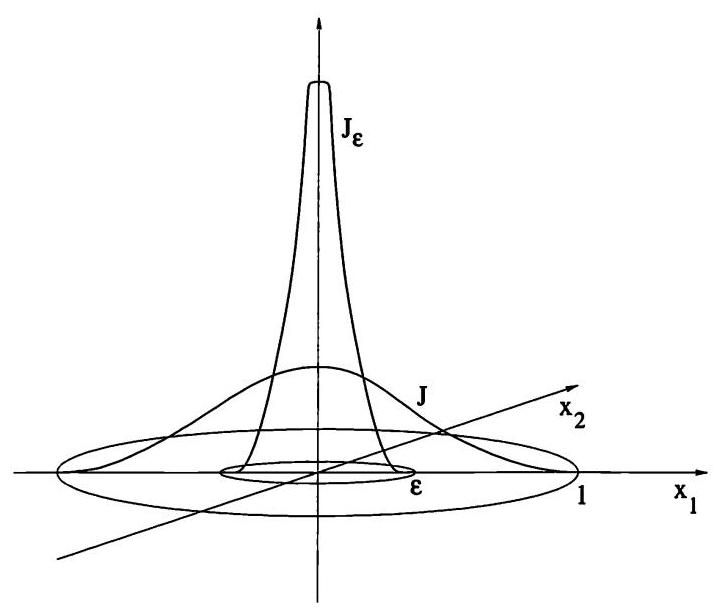
\includegraphics[width=0.6\textwidth]{images/bo_d6ik6nn7aajc739ct1l0_240_398_1533_718_612_0.jpg}
\caption{标准磨光核 $J$ 及其缩放 ${J}_{\varepsilon }$.}
\label{fig:app-A-5-1}
\end{figure}

设 $\Omega  \subseteq  {\mathbb{R}}^{n}$ 为开集， $f \in  {L}_{\text{ loc }}^{1}\left( \Omega \right)$ 为局部可积函数.我们通过卷积定义 $f$ 的磨光:
\[
{f}_{\varepsilon } \doteq  {J}_{\varepsilon } * f
\]

由于 $f$ 定义在 $\Omega$ 上，而 ${J}_{\varepsilon }$ 的支集包含于以原点为中心、半径为 $\varepsilon$ 的球内，该卷积在子集
\[
{\Omega }_{\varepsilon } \doteq  \left\{  {x \in  \Omega ;\overline{B\left( {x,\varepsilon }\right) } \subseteq  \Omega }\right\}  .
\]
中所有点处均有定义.事实上
\[
{f}_{\varepsilon }\left( x\right)  \doteq  {\int }_{B\left( {x,\varepsilon }\right) }{J}_{\varepsilon }\left( {x - y}\right) f\left( y\right) {dy} = {\int }_{B\left( {0,\varepsilon }\right) }{J}_{\varepsilon }\left( z\right) f\left( {x - z}\right) {dz}.
\]

\begin{theorem}[磨光核的性质]\label{thm:app-A-16}
设 $\Omega  \subseteq  {\mathbb{R}}^{n}$ 为开集， $f \in  {L}_{\text{ loc }}^{1}\left( \Omega \right)$ .则:

(i) 对每个 $\varepsilon  > 0$ ，有 ${f}_{\varepsilon } \in  {\mathcal{C}}^{\infty }\left( {\Omega }_{\varepsilon }\right)$ .

(ii) 当 $\varepsilon  \rightarrow  0$ 时，有逐点收敛 ${f}_{\varepsilon }\left( x\right)  \rightarrow  f\left( x\right)$ ，对几乎处处 $x \in  \Omega$ 成立.

(iii) 若 $f$ 连续，则 ${f}_{\varepsilon } \rightarrow  f$ 在 $\Omega$ 的每个紧子集上一致收敛.

(iv) 若 $1 \leq  p < \infty$ 且 $f \in  {L}_{\text{ loc }}^{p}\left( \Omega \right)$ ，则 ${f}_{\varepsilon } \rightarrow  f$ 在 ${L}_{\text{ loc }}^{p}\left( \Omega \right)$ 中成立.
\end{theorem}

\begin{proof}
1. 注意每个 ${\Omega }_{\varepsilon }$ 均为开集.事实上，若闭球 $\overline{B\left( {{x}_{0},\varepsilon }\right) }$ 完全包含于开集 $\Omega$ 中，则当 $\left| {x - {x}_{0}}\right|$ 充分小时，球 $\overline{B\left( {x,\varepsilon }\right) }$ 亦完全包含于 $\Omega$ 中.

设 $\left\{  {{e}_{1},\ldots ,{e}_{n}}\right\}$ 为 ${\mathbb{R}}^{n}$ 的标准标准正交基.固定一点 $x \in  {\Omega }_{\varepsilon }$ 和 $i \in  \{ 1,\ldots ,n\}$ .若 $h$ 足够小，使得 $x + h{e}_{i} \in  {\Omega }_{\varepsilon }$ ，则差商计算为
\begin{align}\tag{A.15}\label{eq:app-A-15}
    &\frac{{f}_{\varepsilon }\left( {x + h{e}_{i}}\right)  - {f}_{\varepsilon }\left( x\right) }{h}\\
    &= \frac{1}{{\varepsilon }^{n}}{\int }_{B\left( {x,\varepsilon }\right) }\frac{1}{h}\left(  {J\left( \frac{x + h{e}_{i} - y}{\varepsilon }\right)  - J\left( \frac{x - y}{\varepsilon }\right) }\right)  f\left( y\right) {dy}.
\end{align}

由于闭球 $\overline{B\left( {x,\varepsilon }\right) }$ 完全包含于 $\Omega$ 中，故有 $f \in \; {L}^{1}\left( {B\left( {x,\varepsilon }\right) }\right)$ .此外，由于 $J \in  {\mathcal{C}}^{\infty }$，我们得到一致收敛
\[
\mathop{\lim }\limits_{{h \rightarrow  0}}\frac{1}{h}\left(  {J\left( \frac{x + h{e}_{i} - y}{\varepsilon }\right)  - J\left( \frac{x - y}{\varepsilon }\right) }\right)   = \frac{1}{\varepsilon }\frac{\partial }{\partial {x}_{i}}J\left( \frac{x - y}{\varepsilon }\right) .
\]

在 \eqref{eq:app-A-15} 式中令 $h \rightarrow  0$ ，可得偏导数的存在性
\[
\frac{\partial }{\partial {x}_{i}}{f}_{\varepsilon }\left( x\right)  = {\int }_{B\left( {x,\varepsilon }\right) }\frac{\partial }{\partial {x}_{i}}{J}_{\varepsilon }\left( {x - y}\right) f\left( y\right) {dy}.
\]

类似论证表明，对任一多重指标 $\alpha$ ，导数 ${D}^{\alpha }{f}_{\varepsilon }$ 存在且
\[
{D}^{\alpha }{f}_{\varepsilon }\left( x\right)  = {\int }_{B\left( {x,\varepsilon }\right) }{D}^{\alpha }{J}_{\varepsilon }\left( {x - y}\right) f\left( y\right) {dy}.
\]

这证明了 (i).

\noindent 2. 由Lebesgue微分定理，对几乎处处的 $x \in  \Omega$ ，有
\begin{equation}\tag{A.16}\label{eq:app-A-16}
\mathop{\lim }\limits_{{r \rightarrow  0}}{f}_{B\left( {x,r}\right) }\left| {f\left( y\right)  - f\left( x\right) }\right| {dy} = 0.
\end{equation}

若 $x$ 是满足 \eqref{eq:app-A-16} 式的点，则
{\begin{align}
    \left| {{f}_{\varepsilon }\left( x\right)  - f\left( x\right) }\right|  &= \left| {{\int }_{B\left( {x,\varepsilon }\right) }{J}_{\varepsilon }\left( {x - y}\right) \left(  {f\left( y\right)  - f\left( x\right) }\right)  {\d y}}\right|\\
    &\leq  \frac{1}{{\varepsilon }^{n}}{\int }_{B\left( {x,\varepsilon }\right) }J\left( \frac{x - y}{\varepsilon }\right) \left| {f\left( y\right)  - f\left( x\right) }\right| {\d y}\\
    &\leq  C{f}_{B\left( {x,\varepsilon }\right) }\left| {f\left( y\right)  - f\left( x\right) }\right| {\d y}.
\end{align}}

当 $\varepsilon  \rightarrow  0$ 时，右端因 \eqref{eq:app-A-16} 而趋于零.这证明了 (ii).

\begin{figure}[htbp]
\centering
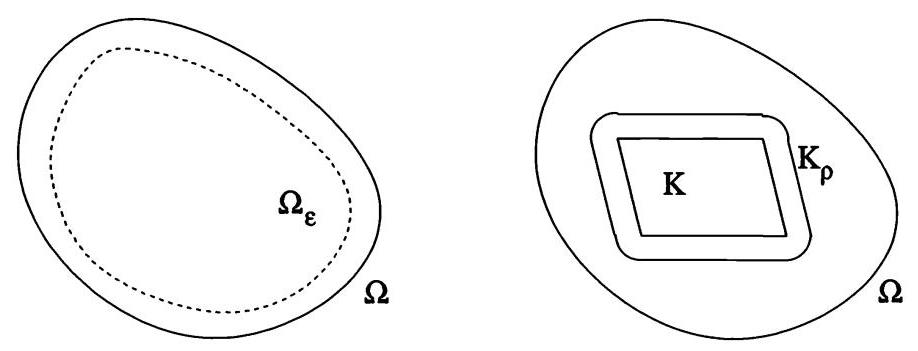
\includegraphics[width=0.8\textwidth]{images/bo_d6ik6nn7aajc739ct1l0_242_301_1360_918_351_0.jpg}
\caption{集合 ${\Omega }_{\varepsilon } \subset  \Omega$ 及紧集 $K \subset   \subset \; {K}_{\rho } \subset   \subset  \Omega$ ，用于磨光子分析.}
\label{fig:app-A-5-2}
\end{figure}

\noindent 3. 假设 $f$ 连续，设 $K \subset  \Omega$ 为一紧子集.则可选取足够小的 $\delta  > 0$ ，使得紧邻域
\begin{equation}\tag{A.17}\label{eq:app-A-17}
{K}_{\rho } \doteq  \left\{  {x \in  {\mathbb{R}}^{n};d\left( {x,K}\right)  \leq  \rho }\right\}
\end{equation}

仍包含于 $\Omega$ 内.由于 $f$ 在紧集 ${K}_{\rho }$ 上一致连续，前述计算表明 ${f}_{\varepsilon }\left( x\right)  \rightarrow  f\left( x\right)$ 对 $x \in  K$ 一致成立.这证明了 (iii).

\noindent 4. 为证明 (iv)，假设 $1 \leq  p < \infty$ 且 $f \in  {L}_{\text{ loc }}^{p}\left( \Omega \right)$ .设 $K \subset  \Omega$ 为一紧子集，并选取 $\rho  > 0$ ，使得 \eqref{eq:app-A-17} 中的紧邻域 ${K}_{\rho }$ 仍包含于 $\Omega$ 内.我们声称:对任意 $0 < \varepsilon  < \rho$ ，有
\begin{equation}\tag{A.18}\label{eq:app-A-18}
{\norm{f}_{\varepsilon }}_{{L}^{p}\left( K\right) } \leq  \| f{\| }_{{L}^{p}\left( {K}_{\rho }\right) }.
\end{equation}

事实上，对 $x \in  K$ ，应用 Hölder 不等式(指数为 $q = \frac{p}{p - 1}$ )可得
{\setjot[-2]\begin{align*}
    \left| {{f}_{\varepsilon }\left( x\right) }\right|  &= \left| {{\int }_{B\left( {x,\varepsilon }\right) }{J}_{\varepsilon }\left( {x - y}\right) f\left( y\right) {\d y}}\right|\\
    &\leq  {\int }_{B\left( {x,\varepsilon }\right) }{\left( {J}_{\varepsilon }\left( x - y\right) \right) }^{\frac{p - 1}{p}}{\left( {J}_{\varepsilon }\left( x - y\right) \right) }^{\frac{1}{p}}\left| {f\left( y\right) }\right| {\d y}\\
    &\leq  {\left( {\int }_{B\left( {x,\varepsilon }\right) }{J}_{\varepsilon }\left( x - y\right) dy\right) }^{\frac{p - 1}{p}}{\left( {\int }_{B\left( {x,\varepsilon }\right) }{J}_{\varepsilon }\left( x - y\right) {\left| f\left( y\right) \right| }^{p}dy\right) }^{\frac{1}{p}}.
\end{align*}}


回顾 ${\int }_{B\left( {x,\varepsilon }\right) }{J}_{\varepsilon }\left( {x - y}\right) {dy} = 1$ ，对 $0 < \varepsilon  < \rho$ ，上述不等式给出
{\setjot[-2]\begin{align*}
    {\int }_{K}{\left| {f}_{\varepsilon }\left( x\right) \right| }^{p}{\d x} &\leq  {\int }_{K}\left( {{\int }_{B\left( {x,\varepsilon }\right) }{J}_{\varepsilon }\left( {x - y}\right) {\left| f\left( y\right) \right| }^{p}{dy}}\right) {\d x}\\
    &\leq  {\int }_{{K}_{\rho }}{\left| f\left( y\right) \right| }^{p}\left( {{\int }_{B\left( {y,\varepsilon }\right) }{J}_{\varepsilon }\left( {x - y}\right) {\d x}}\right) {\d y} = {\int }_{{K}_{\rho }}{\left| f\left( y\right) \right| }^{p}{\d y}.
\end{align*}}

这就证明了 \eqref{eq:app-A-18}.

接下来，对任意 $\delta  > 0$ ，我们选取 $g \in  \mathcal{C}\left( {K}_{\rho }\right)$ 使得
\[
\| f - g{\| }_{{L}^{p}\left( {K}_{\rho }\right) } < \delta
\]

结合\eqref{eq:app-A-18}，可得
{\setjot[-2]\begin{align*}
    {\norm{f_{\varepsilon } - f}}_{{L}^{p}\left( K\right) } &\leq  {\norm{f}_{\varepsilon } - {g}_{\varepsilon }}_{{L}^{p}\left( K\right) } + {\norm{g}_{\varepsilon } - g}_{{L}^{p}\left( K\right) } + \| g - f{\| }_{{L}^{p}\left( K\right) }\\
    &\leq  \| f - g{\| }_{{L}^{p}\left( {K}_{\rho }\right) } + {\norm{g}_{\varepsilon } - g}_{{L}^{p}\left( K\right) } + \| g - f{\| }_{{L}^{p}\left( K\right) }\\
    &\leq  \delta  + {\norm{g}_{\varepsilon } - g}_{{L}^{p}\left( K\right) } + \delta .
\end{align*}}


由于 $g$ 连续，由(ii)可知 $\left| {{g}_{\varepsilon } - g}\right|  \rightarrow  0$ 在紧集 ${K}_{\rho }$ 上一致成立.因此 $\limsup_{{\varepsilon  \rightarrow  0}}{\norm{f_{\varepsilon } - f}}_{{L}^{p}\left( K\right) } \leq  {2\delta }$ .由于 $\delta  > 0$ 是任意的，这便证明了(iv).
\end{proof}

\begin{corollary}\label{cor:app-A-17}
设 $f \in  {L}_{\text{ loc }}^{1}\left( \Omega \right)$ ，并假设
\[
{\int }_{\Omega }{f\phi \d x} = 0,\;\forall\,\phi  \in  {\mathcal{C}}_{\mathrm{c}}^{\infty }\left( \Omega \right) .
\]

则对几乎处处的 $x \in  \Omega$ ，有 $f\left( x\right)  = 0$ .
\end{corollary}

\begin{proof}
事实上，设 $x \in  \Omega$ 为 $f$ 的一个Lebesgue点， ${J}_{\varepsilon }$ 为标准磨光核.取 $\phi \left( y\right)  = {J}_{\varepsilon }\left( {x - y}\right)$，并令 $\varepsilon  \rightarrow  0$，可得
\[
0 = {\int }_{\Omega }{J}_{\varepsilon }\left( {x - y}\right) f\left( y\right) {dy} = {\int }_{B\left( {x,\varepsilon }\right) }J\left( {x - y}\right) f\left( y\right) {dy} \rightarrow  f\left( x\right) .
\]

故对几乎处处的 $x \in  \Omega$ ，有 $f\left( x\right)  = 0$ .
\end{proof}

\subsection{单位分解}
设 $S \subseteq  {\mathbb{R}}^{n}$ ， ${V}_{1},{V}_{2},\ldots$ 为覆盖 $S$ 的一族开集，即
\[
S \subseteq  \mathop{\bigcup }\limits_{{k \geq  1}}{V}_{k}
\]

若一族函数 $\left\{  {{\phi }_{k};k \geq  1}\right\}$ 满足下列条件，则称其为关于集合 ${V}_{k}$ 的光滑单位分解.

(i) 对每个 $k \geq  1,{\phi }_{k} : {\mathbb{R}}^{n} \mapsto  \left(  {0,1}\right)$ ， ${\mathcal{C}}^{\infty }$ 是支撑集包含于开集 ${V}_{k}$ 内的 ${\mathcal{C}}^{\infty }$ 函数.

(ii) 每一点 $x \in  S$ 均存在一个邻域，该邻域仅与有限个函数 ${\phi }_{k}$ 的支撑集相交.此外
\begin{equation}\tag{A.19}\label{eq:app-A-19}
\sum_{k}{\phi }_{k}\left( x\right)  = 1\;\forall\,x \in  S.
\end{equation}

注意，由假设(ii)，在每一点 $x \in  S$ 处，\eqref{eq:app-A-19}式中的求和仅含有限个非零项.

\begin{figure}[htbp]
\centering
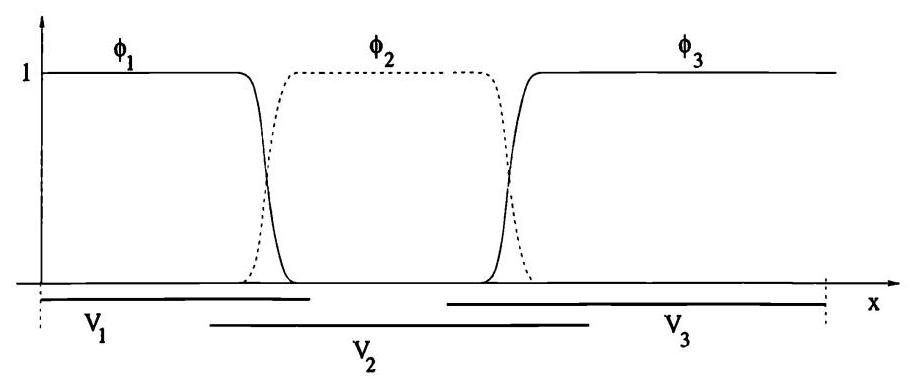
\includegraphics[width=0.8\textwidth]{images/bo_d6ik6nn7aajc739ct1l0_244_301_1743_909_382_0.jpg}
\caption{关于集合 ${V}_{1},{V}_{2},{V}_{3}$ 的单位分解.}
\label{fig:app-A-5-3}
\end{figure}

\begin{theorem}[光滑单位分解的存在性]\label{thm:app-A-18}
设 $S \subseteq \; {\mathbb{R}}^{n}$ ， $\left\{  {{V}_{k};k \geq  1}\right\}$ 为覆盖 $S$ 的一族开集，则存在关于集合 ${V}_{k}$ 的光滑单位分解.
\end{theorem}

\section{不等式}

\subsection{凸集与凸函数}
集合 $\Omega  \subseteq  {\mathbb{R}}^{n}$ 称为凸集，若
\[
x,y \in  \Omega ,\theta  \in  \left(  {0,1}\right)  \implies {\theta x} + \left( {1 - \theta }\right) y \in  \Omega .
\]

换言之，若 $\Omega$ 包含两点 $x,y$ ，则它也包含连接 $x$ 与 $y$ 的整个线段.

设 $\Omega  \subset  {\mathbb{R}}^{n}$ 为一个凸集.若函数 $f : \Omega  \mapsto  \mathbb{R}$ 满足
\begin{equation}\tag{A.20}\label{eq:app-A-20}
f\left( {{\theta x} + \left( {1 - \theta }\right) y}\right)  \leq  {\theta f}\left( x\right)  + \left( {1 - \theta }\right) f\left( y\right)
\end{equation}

对任意 $x,y \in  \Omega$ 和 $\theta  \in  \left(  {0,1}\right)$ 成立，则称其为凸函数.注意，\eqref{eq:app-A-20} 式成立当且仅当 $f$ 的上图(即集合
\[
\{ \left( {x,z}\right)  \in  \Omega  \times  \mathbb{R};z \geq  f\left( x\right) \}
\]
是 ${\mathbb{R}}^{n} \times  \mathbb{R}$ 的一个凸子集.

若二阶可微函数 $f : {\mathbb{R}}^{n} \mapsto  \mathbb{R}$ 的黑塞矩阵(二阶导数矩阵)一致正定，则称其为一致凸函数.这意味着:存在某个常数 $\kappa  > 0$ ，使得
\[
\sum_{{i,j = 1}}^{n}{f}_{{x}_{i}{x}_{j}}\left( x\right) {\xi }_{i}{\xi }_{j} \geq  \kappa \sum_{{i = 1}}^{n}{\xi }_{i}^{2}\;\forall\,x,\xi  \in  {\mathbb{R}}^{n}.
\]

\begin{figure}[htbp]
\centering
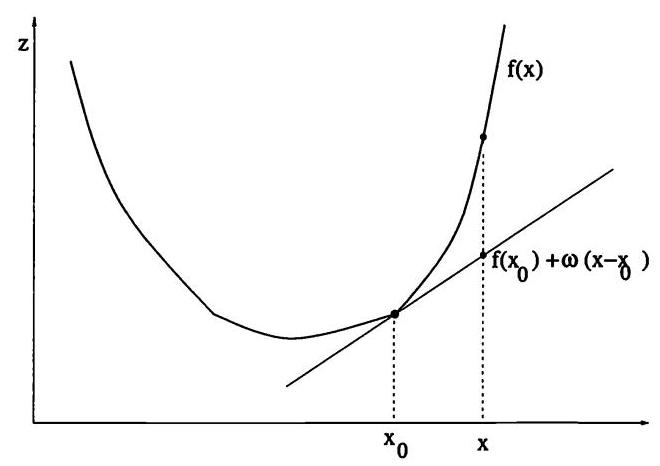
\includegraphics[width=0.6\textwidth]{images/bo_d6ik6nn7aajc739ct1l0_245_426_1636_660_466_0.jpg}
\caption{凸函数 $f$ 及其上图；点 ${x}_{0}$ 处的一个支撑超平面.}
\label{fig:app-A-6-1}
\end{figure}

\begin{theorem}[支撑超平面]\label{thm:app-A-19}
设 $f : {\mathbb{R}}^{n} \mapsto  {\mathbb{R}}^{n}$ 为凸函数，则对每个 ${x}_{0} \in  {\mathbb{R}}^{n}$ ，均存在一个(次梯度)向量 $\omega$ ，使得
\[
f\left( x\right)  \geq  f\left( {x}_{0}\right)  + \left\langle  {\omega ,x - {x}_{0}}\right\rangle  \;\forall\,x \in  {\mathbb{R}}^{n}.
\]

超平面 $\left\{  {\left( {x,z}\right) ;z = \left\langle  {\omega ,x - {x}_{0}}\right\rangle  }\right\}   \subset  {\mathbb{R}}^{n + 1}$ 在点 ${x}_{0}$ 处与 $f$ 的图像相切，且对所有 $x \in  {\mathbb{R}}^{n}$ 均位于该图像下方.因此称其为 $f$ 在 ${x}_{0}$ 处的一个支撑超平面.
\end{theorem}

\begin{theorem}[詹森不等式]\label{thm:app-A-20}
设 $f : \mathbb{R} \mapsto  \mathbb{R}$ 为凸函数， $\Omega  \subset  {\mathbb{R}}^{n}$ 为有界开集.若 $u \in  {L}^{1}\left( \Omega \right)$ 是任一可积函数，则
\begin{equation}\tag{A.21}\label{eq:app-A-21}
f\left( {{\int }_{\Omega }{u\d x}}\right)  \leq  {\oint }_{\Omega }f\left( u\right) {\d x}
\end{equation}
此处 ${f}_{\Omega }{u\d x} \doteq  \frac{1}{\operatorname{meas}\left( \Omega \right) }{\int }_{\Omega }{u\d x}$ 表示 $u$ 在集合 $\Omega$ 上的平均值，而 ${f}_{\Omega }f\left( u\right) {\d x} \doteq  \frac{1}{\operatorname{meas}\left( \Omega \right) }{\int }_{\Omega }f\left( u\right) {\d x}$ 表示 $f\left( u\right)$ 的平均值.注意:我们并不要求集合 $\Omega$ 是凸的.
\end{theorem}

\begin{proof}
令 ${u}_{0} \doteq  {f}_{\Omega }u\left( y\right) {dy}$ .则在点 ${u}_{0}$ 处， $f$ 的图像存在一个支撑超平面，记为 $f\left( u\right)  \geq  f\left( {u}_{0}\right)  + \left\langle  {\omega ,u - {u}_{0}}\right\rangle$ ，其中 $\omega  \in  \mathbb{R}$ 为某常数，且对所有 $u \in  \mathbb{R}$ 成立.故有
\[
f\left( {u\left( x\right) }\right)  \geq  f\left( {{\oint }_{\Omega }u\left( y\right) {dy}}\right) {\d x} + \left\langle  {\omega ,u\left( x\right)  - {\oint }_{\Omega }u\left( y\right) {dy}}\right\rangle  .
\]

对集合 $\Omega$ 上等式两边取平均值，即得 \eqref{eq:app-A-21} 式.
\end{proof}

\subsection{基本不等式.}

\subsubsection{1. Cauchy不等式.}

\begin{equation}\tag{A.22}\label{eq:app-A-22}
{ab} \leq  \frac{{a}^{2} + {b}^{2}}{2}\;\forall\,a,b \in  \mathbb{R}.
\end{equation}

事实上， $0 \leq  {\left( a - b\right) }^{2} = {a}^{2} + {b}^{2} - {2ab}$ .

对任意 $\varepsilon  > 0$ ，在 \eqref{eq:app-A-22} 中将 $a$ 替换为 $\sqrt{2\varepsilon }a$ 、 $b$ 替换为 $b/\sqrt{2\varepsilon }$ ，可得如下稍一般的不等式
\begin{equation}\tag{A.23}\label{eq:app-A-23}
{ab} \leq  \varepsilon {a}^{2} + \frac{{b}^{2}}{4\varepsilon }\;\left( {a,b \in  \mathbb{R},\varepsilon  > 0}\right) .
\end{equation}

\subsubsection*{2. Young不等式.}
\begin{equation}\tag{A.24}\label{eq:app-A-24}
{ab} \leq  \frac{{a}^{p}}{p} + \frac{{b}^{q}}{q}\;\left( {a,b > 0,1 < p < q < \infty ,\frac{1}{p} + \frac{1}{q} = 1}\right) \text{ . }
\end{equation}

事实上，由于映射 $f\left( u\right)  = {e}^{u}$ 是凸的，故有 $\exp \left\{  {\frac{u}{p} + \frac{v}{q}}\right\}   \leq  \frac{{e}^{u}}{p} + \; \frac{{e}^{v}}{q}$ .因此
\[
{ab} = {e}^{\ln a + \ln b} = \exp \left\{  {\frac{1}{p}\ln {a}^{p} + \frac{1}{q}\ln {b}^{q}}\right\}   \leq  \frac{1}{p}{e}^{\ln {a}^{p}} + \frac{1}{q}{e}^{\ln {b}^{q}} = \frac{{a}^{p}}{p} + \frac{{b}^{q}}{q}.
\]

\subsubsection*{3. Hölder不等式.}若 $f \in  {L}^{p}\left( \Omega \right) ,g \in  {L}^{q}\left( \Omega \right)$ ，且 $1 \leq  p,q \leq  \infty$ 、 $\frac{1}{p} + \frac{1}{q} = 1$ ，则
\begin{equation}\tag{A.25}\label{eq:app-A-25}
{\int }_{\Omega }\left| {fg}\right| {\d x} \leq  \| f{\| }_{{L}^{p}\left( \Omega \right) }\| g{\| }_{{L}^{q}\left( \Omega \right) }.
\end{equation}

事实上，在 $\| f{\| }_{{L}^{p}\left( \Omega \right) } = \| g{\| }_{{L}^{q}\left( \Omega \right) } = 1$ 的特殊情形下，杨不等式给出
\[
{\int }_{\Omega }\left| {fg}\right| {\d x} \leq  \frac{1}{p}{\int }_{\Omega }{\left| f\right| }^{p}{\d x} + \frac{1}{q}{\int }_{\Omega }{\left| g\right| }^{q}{\d x} = \frac{1}{p} + \frac{1}{q} = 1 = \| f{\| }_{{L}^{p}}\| g{\| }_{{L}^{q}}.
\]

为涵盖一般情形，我们只需将函数 $f,g$ 分别替换为 $\widetilde{f} = \; f/\| f{\| }_{{L}^{p}}$ 和 $\widetilde{g} = g/\| g{\| }_{{L}^{q}}$ .

通过归纳法，可建立Hölder不等式的如下更一般形式:设 $1 \leq  {p}_{1},\ldots ,{p}_{m} \leq  \infty$ ，且 $\frac{1}{{p}_{1}} + \cdots  + \frac{1}{{p}_{m}} = 1$ ；假设对所有 $k = 1,\ldots ,m$ 均有 ${f}_{k} \in  {L}^{{p}_{k}}\left( \Omega \right)$ ，则
\begin{equation}\tag{A.26}\label{eq:app-A-26}
{\int }_{\Omega }\left| {{f}_{1}{f}_{2}\cdots {f}_{m}}\right| {\d x} \leq  \mathop{\prod }\limits_{{k = 1}}^{m}{\norm{f}_{k}}_{{L}^{{p}_{k}}\left( \Omega \right) }.
\end{equation}

\subsubsection*{4. Minkowski不等式.}对任意 $1 \leq  p \leq  \infty$ 和 $f,g \in  {L}^{p}\left( \Omega \right)$ ，有
\begin{equation}\tag{A.27}\label{eq:app-A-27}
\| f + g{\| }_{{L}^{p}\left( \Omega \right) } \leq  \| f{\| }_{{L}^{p}\left( \Omega \right) } + \| g{\| }_{{L}^{p}\left( \Omega \right) }.
\end{equation}

事实上，当 $p = 1$ 时，结论显然成立；若 $p > 1$ ，将指数分别为 $p$ 和 $q = \frac{p}{p - 1}$ 的Hölder不等式应用于该情形，可得
{\begin{align*}
    {\| f + g\| }_{{L}^{p}\left( \Omega \right) }^{p} &= {\int }_{\Omega }{\left| f + g\right| }^{p}{\d x} = {\int }_{\Omega }{\left| f + g\right| }^{p - 1}\left( {\left| f\right|  + \left| g\right| }\right) {\d x}\\
    &\leq  {\left( {\int }_{\Omega }{\left| f + g\right| }^{\left( {p - 1}\right)  \cdot  \frac{p}{p - 1}}\d x\right) }^{\frac{p - 1}{p}}\left(  {{\left( {\int }_{\Omega }{\left| f\right| }^{p}\d x\right) }^{\frac{1}{p}} + {\left( {\int }_{\Omega }{\left| g\right| }^{p}\d x\right) }^{\frac{1}{p}}}\right) \\
    &= \| f + g{\| }_{{L}^{p}\left( \Omega \right) }^{p - 1}\left( {\| f{\| }_{{L}^{p}\left( \Omega \right) } + \| g{\| }_{{L}^{p}\left( \Omega \right) }}\right) .
\end{align*}}


两边同除以 $\| f + g{\| }_{{L}^{p}\left( \Omega \right) }^{p - 1}$ ，即得\eqref{eq:app-A-27}.

\subsubsection*{5. 插值不等式.}设 $1 \leq  p \leq  r \leq  q \leq  \infty$ ，且满足
\[
\frac{1}{r} = \frac{\theta }{p} + \frac{1 - \theta }{q}\;\text{ 对某个 }\theta  \in  \left(  {0,1}\right)  .
\]

若 $f \in  {L}^{p}\left( \Omega \right)  \cap  {L}^{q}\left( \Omega \right)$ ，则还有 $f \in  {L}^{r}\left( \Omega \right)$ ，且
\begin{equation}\tag{A.28}\label{eq:app-A-28}
\| f{\| }_{{L}^{r}\left( \Omega \right) }\; \leq  \;\| f{\| }_{{L}^{p}\left( \Omega \right) }^{\theta }\| f{\| }_{{L}^{q}\left( \Omega \right) }^{1 - \theta }.
\end{equation}

事实上，注意到 $\frac{\theta r}{p} + \frac{\left( {1 - \theta }\right) r}{q} = 1$ ，由Hölder不等式可得
\begin{align*}
    {\int }_{\Omega }{\left| f\right| }^{r}{\d x} &= {\int }_{\Omega }{\left| f\right| }^{\theta r}{\left| f\right| }^{\left( {1 - \theta }\right) r}{\d x}\\
    &\leq  {\left( {\int }_{\Omega }{\left| f\right| }^{{\theta r} \cdot  \tfrac{p}{{\theta }_{r}}}\d x\right) }^{\tfrac{{\theta }_{r}}{p}}{\left( {\int }_{\Omega }{\left| f\right| }^{\left( {1 - \theta }\right) r \cdot  \tfrac{q}{\left( {1 - \theta }\right) r}}\d x\right) }^{\tfrac{\left( {1 - \theta }\right) r}{q}}
\end{align*}


\subsubsection*{6. 离散型Hölder与Minkowski不等式.}不等式\eqref{eq:app-A-25}与\eqref{eq:app-A-27}更一般地在 $\Omega$ 为任意测度空间时仍成立.特别地，可取 $\Omega  = \{ 1,\ldots ,n\}$ 并赋予计数测度.对任意数组 ${a}_{1},\ldots ,{a}_{n}$ 与 ${b}_{1},\ldots ,{b}_{n}$ ，以及满足 $\frac{1}{p} + \frac{1}{q} = 1$ 的 $1 \leq  p,q < \infty$ ，有离散型Hölder不等式
\begin{equation}\tag{A.29}\label{eq:app-A-29}
\sum_{{k = 1}}^{n}\left| {{a}_{k}{b}_{k}}\right|  \leq  {\left( \sum_{{k = 1}}^{n}{\left| {a}_{k}\right| }^{p}\right) }^{\frac{1}{p}}{\left( \sum_{{k = 1}}^{n}{\left| {b}_{k}\right| }^{q}\right) }^{\frac{1}{q}}
\end{equation}
及离散型Minkowski不等式
\begin{equation}\tag{A.30}\label{eq:app-A-30}
{\left( \sum_{{k = 1}}^{n}{\left| {a}_{k} + {b}_{k}\right| }^{p}\right) }^{\frac{1}{p}} \leq  {\left( \sum_{{k = 1}}^{n}{\left| {a}_{k}\right| }^{p}\right) }^{\frac{1}{p}} + {\left( \sum_{{k = 1}}^{n}{\left| {b}_{k}\right| }^{p}\right) }^{\frac{1}{p}}
\end{equation}

给定两个向量 $x = \left( {{x}_{1},\ldots ,{x}_{n}}\right)$ 和 $y = \left( {{y}_{1},\ldots ,{y}_{n}}\right)$ ，在 $p = q = 2$ 下应用离散 Hölder 不等式\eqref{eq:app-A-29}，可得定义在 ${\mathbb{R}}^{n}$ 上的内积的 Cauchy-Schwarz 不等式:
\begin{equation}\tag{A.31}\label{eq:app-A-31}
\left| {\langle x,y\rangle }\right|  \leq  \left| x\right| \left| y\right| .
\end{equation}

事实上，
\[
\left| {\langle x,y\rangle }\right|  = \left| {\sum_{{k = 1}}^{n}{x}_{k}{y}_{k}}\right|  \leq  \sum_{{k = 1}}^{n}\left| {{x}_{k}{y}_{k}}\right|  \leq  {\left( \sum_{{k = 1}}^{n}{\left| {x}_{k}\right| }^{2}\right) }^{\frac{1}{2}}{\left( \sum_{{k = 1}}^{n}{\left| {y}_{k}\right| }^{2}\right) }^{\frac{1}{2}} = \left| x\right| \left| y\right| .
\]

\subsection{一个微分不等式.}

\begin{theorem}[Gronwall 不等式]\label{thm:app-A-21}
设 $t \mapsto  z\left( t\right)$ 是定义在 $t \in  \left(  {0,T}\right)$ 上的非负绝对连续函数.假设其时间导数 ${z}^{\prime } = \frac{\d}{\d t}z$ 满足
\[
{z}^{\prime }\left( t\right)  \leq  \phi \left( t\right) z\left( t\right)  + \psi \left( t\right) \;\text{ for a.e. }t \in  \left(  {0,T}\right)  ,
\]

其中 $\phi ,\psi  \in  {L}^{1}\left( \left(  {0,T}\right)  \right)$ 为非负函数.则有\eqref{eq:app-A-32}
\begin{equation}\tag{A.32}\label{eq:app-A-32}
z\left( t\right) \; \leq  \;{e}^{{\int }_{0}^{t}\phi \left( s\right) \;{ds}}z\left( 0\right) \; + \;{\int }_{0}^{t}{e}^{{\int }_{s}^{t}\phi \left( \sigma \right) \;{d\sigma }}\psi \left( s\right){\d s}\;\forall\,\;t \in  \left(  {0,T}\right)  .
\end{equation}
\end{theorem}

\begin{proof}
注意，\eqref{eq:app-A-32} 右端恰好是初值问题
\[
{Z}^{\prime }\left( t\right)  = \phi \left( t\right) Z\left( t\right)  + \psi \left( t\right) ,\;Z\left( 0\right)  = z\left( 0\right) .
\]

为证明 \eqref{eq:app-A-32}，我们写出
\[
\frac{\d}{\d s}\left( {{e}^{-{\int }_{0}^{s}\phi \left( \sigma \right) \;{d\sigma }}z\left( s\right) }\right) \; = \;{e}^{-{\int }_{0}^{s}\phi \left( \sigma \right) \;{d\sigma }}\left( {{z}^{\prime }\left( s\right)  - \phi \left( s\right) z\left( s\right) }\right) \; \leq  \;{e}^{-{\int }_{0}^{s}\phi \left( \sigma \right) \;{d\sigma }}\psi \left( s\right) .
\]

在区间 $\left(  {0,t}\right)$ 上积分，得
\[
{e}^{-{\int }_{0}^{t}\phi \left( \sigma \right) {d\sigma }}z\left( t\right)  - z\left( 0\right)  \leq  {\int }_{0}^{t}{e}^{-{\int }_{0}^{s}\phi \left( \sigma \right) {d\sigma }}\psi \left( s\right) {\d s}.
\]

两边同乘 ${e}^{{\int }_{0}^{t}\phi \left( \sigma \right) {\d \sigma }}$ ，即得 \eqref{eq:app-A-32}.
\end{proof}

\section{习题}

\begin{rbhw}[index=1]
设 $\left\{  {{A}_{i};i \in  \mathcal{I}}\right\}$ 是紧致度量空间 $K$ 的一个开覆盖.证明存在 $\rho  > 0$ ，使得对任意 $x \in  K$ ，球 $B\left( {x,\rho }\right)$ 完全包含于某个集合 ${A}_{i}$ 中.
\end{rbhw}

\begin{rbhw}
    设 ${\left( {x}_{n}\right) }_{n \geq  1}$ 是度量空间 $E$ 中的一列点.证明下列命题.
    \begin{enumerate}[(i)]
        \item 该序列收敛于某点 $\bar{x}$ 当且仅当从任意子列 ${\left( {x}_{{n}_{j}}\right) }_{j \geq  1}$ 中均可再选出一个收敛于 $\bar{x}$ 的子列.
        \item 若对所有 $m \neq  n$ 均有 $d\left( {{x}_{m},{x}_{n}}\right)  \geq  \delta  > 0$ ，则不存在收敛子列.
        \item 设 $E$ 是完备的，且假设对任意 $\varepsilon  > 0$ ，从任一序列中均可再选出一个子列 ${\left( {x}_{{n}_{j}}\right) }_{j \geq  1}$，使得
\[
\limsup_{{j,k \rightarrow  \infty }}d\left( {{x}_{{n}_{j}},{x}_{{n}_{k}}}\right)  < \varepsilon
\]
则该序列存在收敛子列.
    \end{enumerate}
\end{rbhw}


\begin{rbhw}
考虑函数
\[
f\left( x\right)  = \left\{  \begin{matrix} \frac{1}{x{\left( \ln x\right) }^{2}} & \text{ if }0 < x < \frac{1}{2}, \\  0 & \text{ otherwise. } \end{matrix}\right.
\]

设 ${f}_{\varepsilon } \doteq  {J}_{\varepsilon } * f$ 为其对应的磨光函数，并令
\[
F\left( x\right)  \doteq  \mathop{\sup }\limits_{{0 < \varepsilon  < 1}}{f}_{\varepsilon }\left( x\right)
\]

证明 $f \in  {L}^{1}\left( \mathbb{R}\right)$ 成立，但 $F \notin  {L}^{1}\left( \mathbb{R}\right)$ 不成立.因此，尽管 ${f}_{\varepsilon } \rightarrow  f$ 逐点成立，却无法利用Lebesgue控制收敛定理证明 ${\norm{f}_{\varepsilon } - f}_{{L}^{1}\left( \mathbb{R}\right) } \rightarrow  0$ .
\end{rbhw}

\begin{rbhw}
设 ${f}_{n} : \mathbb{R} \mapsto  \mathbb{R},n \geq  1$ 为一列绝对连续函数，满足
\begin{enumerate}[(i)]
    \item 在点 $x = 0$ 处，序列 ${f}_{n}\left( 0\right)$ 有界；
    \item 存在函数 $g \in  {L}^{1}\left( \mathbb{R}\right)$ ，使得其导数 ${f}_{n}^{\prime }$ 对每个 $n \geq  1$ 及几乎处处 $x \in  \mathbb{R}.$ 满足 $\left| {{f}_{n}^{\prime }\left( x\right) }\right|  \leq  g\left( x\right)$ .
\end{enumerate}
证明:存在子列 ${\left( {f}_{{n}_{j}}\right) }_{j \geq  1}$ ，在全体实轴上一致收敛.
\end{rbhw}

\begin{rbhw}
考虑一列函数 ${f}_{n} \in  {L}^{1}\left( \mathbb{R}\right)$ ，满足对每个 $n \geq  1$ 均有 ${\norm{f}_{n}}_{{L}^{1}} \leq  C$ .定义
\[
f\left( x\right)  \doteq  \left\{  \begin{matrix} \mathop{\lim }\limits_{{n \rightarrow  \infty }}{f}_{n}\left( x\right) & \text{ if the limit exists, } \\  0 & \text{ otherwise. } \end{matrix}\right.
\]

证明: $f$ 是Lebesgue可测的，且 $\| f{\| }_{{L}^{1}} \leq  C$ .
\end{rbhw}

\begin{rbhw}
设 $f : \mathbb{R} \rightarrow  \mathbb{R}$ 为绝对连续函数.证明: $f$ 将Lebesgue测度为零的集合映为Lebesgue测度为零的集合.
\end{rbhw}

\begin{rbhw}
(i) 若 ${\left( {f}_{n}\right) }_{n \geq  1}$ 是 ${L}^{1}\left( \left(  {0,1}\right)  \right)$ 中的一列函数，且满足 ${\norm{f}_{n}}_{{L}^{1}} \rightarrow  0$ ，则证明存在一子列在几乎处处 $x \in  \left(  {0,1}\right)$ 点态收敛.


(ii) 构造一列可测函数 ${f}_{n} : \left(  {0,1}\right)   \mapsto  \left(  {0,1}\right)$ ，使得 ${\norm{f}_{n}}_{{L}^{1}} \rightarrow  0$ 成立，但对每个 $x \in  \left(  {0,1}\right)$，序列 ${f}_{n}\left( x\right)$ 均无极限.
\end{rbhw}

\begin{rbhw}
对任意(非空)开集 $\Omega  \subseteq  {\mathbb{R}}^{n}$ 及 $1 \leq  p \leq  \infty$ ，证明空间 ${L}^{p}\left( \Omega \right)$ 是无限维的.构造一列函数 ${\left( {f}_{j}\right) }_{j \geq  1}$ ，使得
\[
{\norm{f}_{j}}_{{L}^{p}} = 1,\;{\norm{f}_{i} - {f}_{j}}_{{L}^{p}} \geq  1\;\forall\,i,j \geq  1,i \neq  j.
\]
\end{rbhw}

\begin{rbhw}
考虑集合 ${\mathbb{R}}^{2}$ ，其上赋予偏序关系
\[
x \preccurlyeq  y \iff {x}_{1} \leq  {y}_{1}\text{ and }{x}_{2} \leq  {y}_{2}.
\]

设 $f : \mathbb{R} \mapsto  \mathbb{R}$ 为连续、非减函数.证明集合
\[
S \doteq  \operatorname{Graph}\left( f\right)  = \{ \left( {t,f\left( t\right) }\right) ;t \in  \mathbb{R}\}
\]

是 ${\mathbb{R}}^{2}$ 的一个极大全序子集.是否每个极大全序子集均可由此方式得到？
\end{rbhw}

\begin{rbhw}
给出广义Hölder不等式\eqref{eq:app-A-26}的证明.
\end{rbhw}

\chapter{符号说明汇总}

$\mathbb{R}$ ，实数域.

$\mathbb{C}$ ，复数域.

$\mathbb{K}$ ，一个数域，为 $\mathbb{R}$ 或 $\mathbb{C}$ .

Re $z$ 和 $\operatorname{Im}z$ ，复数 $z$ 的实部与虚部.

$\bar{z} = a - {ib}$ ，数 $z = a + {ib} \in  \mathbb{C}$ 的复共轭.

$\left(  {a,b}\right)$ ，闭区间； $( a,b\left(  \text{ , an open interval; }\right)  a,b( ,) a,b)$ 为半开区间.

${\mathbb{R}}^{n}$ ， $n$ 维欧几里得空间.

$\langle  \cdot  , \cdot  \rangle$ ，欧几里得空间 ${\mathbb{R}}^{n}$ 上的标量积.

$\left| v\right|  \doteq  \sqrt{\langle v,v\rangle }$ ，向量 $v \in  {\mathbb{R}}^{n}$ 的欧几里得长度.

$A \setminus  B \doteq  \{ x \in  A,x \notin  B\}$ ，集合的差集.

$\bar{A}$ ，集合 $A$ 的闭包.

$\partial A$ ，集合 $A$ 的边界.

${\Omega }^{\prime } \subset   \subset  \Omega$ ， ${\Omega }^{\prime }$ 的闭包是 $\Omega$ 的紧子集.

${\chi }_{A}$ ，集合 $A.{\chi }_{A}\left( x\right)  = \left\{  \begin{array}{ll} 1 & \text{ if }x \in  A, \\  0 & \text{ if }x \notin  A. \end{array}\right.$ 的示性函数.

$f : A \mapsto  B$ ，从集合 $A$ 到集合 $B$ 的映射.

$a \mapsto  b = f\left( a\right)$ ，函数 $f$ 将元素 $a \in  A$ 映为元素 $b \in  B$ .

$\doteq$ ，定义相等.

$\Leftrightarrow$ ，当且仅当.

$\mathcal{C}\left( E\right)  = \mathcal{C}\left( {E,\mathbb{R}}\right)$ ，度量空间 $E$ 上所有连续实值函数构成的向量空间.

$\mathcal{C}\left( {E,\mathbb{C}}\right)$ ，度量空间 $E$ 上所有连续复值函数构成的向量空间.

$\mathcal{B}C\left( E\right)$ ， $f : E \mapsto \; \mathbb{R}$ 上所有有界连续实值函数构成的空间，其范数为 $\| f\|  = \mathop{\sup }\limits_{{x \in  E}}\left| {f\left( x\right) }\right|$ .

${\ell }^{1},{\ell }^{p},{\ell }^{\infty }$ ，实数(或复数)序列空间.

${L}^{1}\left( \Omega \right) ,{L}^{p}\left( \Omega \right) ,{L}^{\infty }\left( \Omega \right)$ ，Lebesgue空间.

${W}^{k,p}\left( \Omega \right)$ ，Soblev空间，即定义在某个开集 $\Omega  \subseteq  {\mathbb{R}}^{n}$ 上的函数空间，其阶数不超过 $k$ 的弱偏导数属于 ${L}^{p}\left( \Omega \right)$ .
\[
{H}^{k}\left( \Omega \right)  = {W}^{k,2}\left( \Omega \right) \text{ , Hilbert-Soblev 空间. }
\]

${\mathcal{C}}^{k,\gamma }\left( \Omega \right)$ ，Hölder空间，即函数 $u : \Omega  \mapsto  \mathbb{R}$ 构成的空间，其阶数不超过 $k$ 的导数具有指数为 $\gamma  \in  (0,1)$ 的Hölder连续性.

$\|  \cdot  \|  = \|  \cdot  {\| }_{X}$ ，向量空间 $X$ 上的范数.

$\left( {\cdot , \cdot  }\right)  = {\left( \cdot , \cdot  \right) }_{H}$ ，Hilbert空间 $H$ 上的内积.

${X}^{ * }$ ， $X$ 的对偶空间，即所有连续线性泛函 ${x}^{ * } : X \mapsto  \mathbb{K}$ 构成的空间.

$\left\langle  {{x}^{ * },x}\right\rangle   = {x}^{ * }\left( x\right)$ ， ${x}^{ * } \in  {X}^{ * }$ 与 $x \in  X$ 之间的对偶积.

${x}_{n} \rightarrow  x$ ，按范数强收敛；即 $\norm{{x}_{n} - x} \rightarrow  0$ .

${x}_{n} \rightharpoonup  x$ ，弱收敛.

${\varphi }_{n}\overset{ * }{ \rightharpoonup  }\varphi$ ，弱*收敛.

$f * g$ ，两个函数 $f,g : {\mathbb{R}}^{n} \mapsto  \mathbb{R}$ 的卷积.

$\nabla u = \left( {{u}_{{x}_{1}},{u}_{{x}_{2}},\ldots ,{u}_{{x}_{n}}}\right)$ ，函数 $u : {\mathbb{R}}^{n} \mapsto  \mathbb{R}$ 的梯度.

${D}^{\alpha } = {\left( \frac{\partial }{\partial {x}_{1}}\right) }^{{\alpha }_{1}}{\left( \frac{\partial }{\partial {x}_{2}}\right) }^{{\alpha }_{2}}\cdots {\left( \frac{\partial }{\partial {x}_{n}}\right) }^{{\alpha }_{n}} = {\partial }_{{x}_{1}}^{{\alpha }_{1}}{\partial }_{{x}_{2}}^{{\alpha }_{2}}\cdots {\partial }_{{x}_{n}}^{{\alpha }_{n}}$ ，一个阶数为 $\left| \alpha \right|  \doteq  {\alpha }_{1} + {\alpha }_{2} + \cdots  + {\alpha }_{n}$ 的偏微分算子.

meas $\left( \Omega \right)$ ，集合 $\Omega  \subset  {\mathbb{R}}^{n}$ 的Lebesgue测度.

${f}_{\Omega }{f\d x} = \frac{1}{\operatorname{meas}\left( \Omega \right) }{\int }_{\Omega }{f\d x}$ ， $f$ 在集合 $\Omega$ 上的平均值.
